\documentclass{article}
\usepackage[utf8]{inputenc}
\usepackage{tabularx} % extra features for tabular environment
\usepackage{amsmath}  % improve math presentation
\usepackage{graphicx} % takes care of graphic including machinery
\usepackage{xspace}
\usepackage{tikz}
\usepackage{enumitem}
\usetikzlibrary{babel}
\usepackage[american]{circuitikz}
\usetikzlibrary{calc}
\usepackage{float}
\usepackage{siunitx}
\usepackage{pgfplots}
\usepackage{amsfonts} 
\usetikzlibrary{intersections}
\usepgfplotslibrary{fillbetween}
\usepackage[skins,theorems]{tcolorbox}
\tcbset{highlight math style={enhanced,
  colframe=red,colback=white,arc=0pt,boxrule=1pt}}
\pgfplotsset{width=10cm,compat=1.9}
\usepackage[margin=1in,letterpaper]{geometry} % decreases margins
\usepackage{cite} % takes care of citations
\usepackage[final]{hyperref} % adds hyper links inside the generated PDF file
\hypersetup{
colorlinks=true,       % false: boxed links; true: colored links
linkcolor=blue,        % color of internal links
citecolor=blue,        % color of links to bibliography
filecolor=magenta,     % color of file links
urlcolor=blue        
}

\begin{document}

\title{\textbf{CONVEX OPTIMISATION}\\{\textbf{ASSIGNMENT }}}
\author{\textbf{TADIPATRI UDAY KIRAN REDDY}\\\textbf{EE19BTECH11038}}
\maketitle

\section*{\hfil Question 1}
\subsection*{(a)}
Problem (1) is convex.(Positive sum of norm functions is convex)\\
Problem (2) is convex.(Norm is convex and Norm ball is convex)\\
Problem (3) is convex.(Positive sum of norm function is convex)\\
Problem (4) is convex.(Norm is convex and Norm ball is convex)
\subsection*{(b)}
\begin{gather*}
	\nabla Objective = \left(\partial \frac{\overline{x}^T(\mathbf{A}^T\mathbf{A}+\alpha \mathbf{I})\overline{x} - \overline{y}^T\mathbf{A}\overline{x} + \overline{y}^T\overline{y}}{\partial \overline{x}}\right)^T\\
	\implies \nabla Objective = 2(\mathbf{A}^T\mathbf{A}+\alpha \mathbf{I})\overline{x} - 2\overline{y}^T\mathbf{A}
\end{gather*}
\subsection*{(c)}
\begin{gather*}
	\Delta Objective = 0\\
	\implies \overline{x}^* = (\mathbf{A}^T\mathbf{A}+\alpha \mathbf{I})^{-1}\mathbf{A}^T\overline{y}
\end{gather*}
\subsection*{(d)}
Given, $||(\mathbf{A}^T\mathbf{A}+\alpha \mathbf{I})^{-1}\mathbf{A}^T\overline{y}||_2 \le 1$\\
\begin{gather*}
\mathbf{A}^T\left(\overline{y}-\mathbf{A}\overline{x_1^*}\right) = \mathbf{A}^T\left(\overline{y}-\mathbf{A}(\mathbf{A}^T\mathbf{A}+\alpha \mathbf{I})^{-1}\mathbf{A}^T\overline{y}\right) = \mathbf{A}^T\overline{y}-\left(\mathbf{A}^T\mathbf{A} + \alpha I\right)(\mathbf{A}^T\mathbf{A}+\alpha \mathbf{I})^{-1}\mathbf{A}^T\overline{y} + \alpha(\mathbf{A}^T\mathbf{A}+\alpha \mathbf{I})^{-1}\mathbf{A}^T\overline{y}\\
\implies \mathbf{A}^T\left(\overline{y}-\mathbf{A}\overline{x_1^*}\right) = \alpha(\mathbf{A}^T\mathbf{A}+\alpha \mathbf{I})^{-1}\mathbf{A}^T\overline{y}
\implies ||\mathbf{A}^T\left(\overline{y}-\mathbf{A}\overline{x_1^*}\right)||_2 \le \alpha
\end{gather*}
Thus $\overline{x_1}^*$ is a feasible point in Problem (2). Therefore the cost with this point will always be less than optimal cost, $\implies ||\overline{x_2}^*||_2 \le ||\overline{x_1}^*||_2$
\subsection*{(e)}

\section*{\hfil Question 2}
\subsection*{$f_2(\overline{x}) = \sum_{i}||\mathbf{A_i}\overline{x} - \overline{b}||_2$}
Apply epigraph trick on the objective,
\begin{gather*}
	||\mathbf{A_i}\overline{x} - \overline{b}||_2 \le t_i\\
	\begin{aligned}
		\min \quad & \overline{1}^T\overline{t}\\
		\textrm{s.t} \quad & ||\mathbf{A_i}\overline{x} - \overline{b}||_2 \le t_i
	\end{aligned}
\end{gather*}
The above is in form of \textit{SOCP}.
\subsection*{$f_1(\overline{x}) = \sum_{i}||\mathbf{A_i}\overline{x} - \overline{b}||_1$}
\begin{gather*}
	||\mathbf{A_i}\overline{x} - \overline{b}||_1 \le \overline{1}^T\overline{t_i}\\
	\implies \mathbf{A_i}\overline{x} - \overline{b} \le \overline{t_i}; \mathbf{A_i}\overline{x} - \overline{b} \ge -\overline{t_i}\\
	\begin{aligned}
		\min \quad & \sum_{i}\overline{1}^T\overline{t_i} \equiv T\overline{1}\\
		\textrm{s.t} \quad & \mathbf{A_i}\overline{x} - \overline{b} \le \overline{t_i}\\
		& \mathbf{A_i}\overline{x} - \overline{b} \ge -\overline{t_i}
	\end{aligned}
\end{gather*}
The above formulation is a \textit{LP}.
\subsection*{$f_\infty(\overline{x}) = \sum_{i}||\mathbf{A_i}\overline{x} - \overline{b}||_\infty$}
\begin{gather*}
	||\mathbf{A_i}\overline{x} - \overline{b}||_\infty \le t_i\\
	\implies \mathbf{A_i}\overline{x} - \overline{b} \le \overline{1}t_i; \mathbf{A_i}\overline{x} - \overline{b} \ge -\overline{1}t_i\\
	\begin{aligned}
		\min \quad & \overline{1}^T\overline{t} \\
		\textrm{s.t} \quad & \mathbf{A_i}\overline{x} - \overline{b} \le \overline{t_i}\\
		& \mathbf{A_i}\overline{x} - \overline{b} \ge -\overline{t_i}
	\end{aligned}
\end{gather*}
The above formulation is a \textit{LP}.
\section*{\hfil Question 3}
\subsection*{(a)}
To prove that the objective function is quasi-concave we ned to show that all $\alpha$ level supersets are convex.
	\begin{gather*}
		\frac{\overline{\mu}^T\overline{x}}{||\mathbf{V}\overline{x}||_2} \ge \alpha\\
		\implies ||\mathbf{V}\overline{x}||_2 \le \frac{1}{\alpha}\overline{\mu}^T\overline{x}
	\end{gather*}
	Given that $\mathbf{V}$ is symmentric which means quadratic part is convex and the above constarints look like SOCP constraints thus it is convex.
\subsection*{(b)}
\begin{gather*}
	\overline{z} = \frac{\overline{x}}{\overline{\mu}^T\overline{x}}\\\implies
	\frac{\overline{z}}{\overline{1}^T\overline{z}} = \frac{\frac{\overline{x}}{\overline{\mu}^T\overline{x}}}{\frac{\overline{1}^T\overline{x}}{\overline{\mu}^T\overline{x}}}\\
	\implies \tcbhighmath[drop fuzzy shadow]{\overline{x} = \frac{\overline{z}}{\overline{1}^T\overline{z}}}\\
	\frac{\overline{\mu}^T\overline{x}}{||\mathbf{V}\overline{x}||_2} = \frac{\overline{\mu}^T\frac{\overline{z}}{\overline{1}^T\overline{z}}}{||\mathbf{V}\frac{\overline{z}}{\overline{1}^T\overline{z}}||_2} = \frac{sgn\left(\overline{1}^T\overline{z}\right)}{||\mathbf{V}\overline{z}||_2}
\end{gather*}
Given $\overline{\mu}^T\overline{x} \ge 0$ and $\overline{1}^T\overline{x} = 1$ which means $\overline{1}^T\overline{z} = \frac{1}{\overline{\mu}^T\overline{x}} > 0$.
\begin{gather*}
	\implies \tcbhighmath[drop fuzzy shadow]{\frac{\overline{\mu}^T\overline{x}}{||\mathbf{V}\overline{x}||_2} = \frac{1}{||\mathbf{V}\overline{z}||_2}}\\
	||\overline{x}||_1 \le L \implies ||\frac{\overline{z}}{\overline{1}^T\overline{z}}||_1 \le L\\
	{||\overline{z}||_1} \le L{\overline{1}^T\overline{z}}
\end{gather*}
Now transformed problem is,
\begin{gather*}
	\begin{aligned}
		\min \quad & ||\mathbf{V}\overline{z}||_2\\
		\textrm{s.t} \quad & {||\overline{z}||_1} \le L{\overline{1}^T\overline{z}}\\
		& \overline{1}^T\overline{z} \ge 0
	\end{aligned}
\end{gather*}
The above transformed problem has both convex objective and constraints thus it is convex optimisation problem.
\section*{\hfil Question 4}
\subsection*{(a)}
\textit{Lemma:} $(\mathbf{A} + \mathbf{B})^{-1} = \mathbf{A}^{-1} - (I + \mathbf{A}^{-1}\mathbf{B})^{-1}\mathbf{A}^{-1}\mathbf{B}\mathbf{A}^{-1}$.\\
If $g(x)$ is convex then so is $\overline{a}^Tg(x)\overline{a}$ because the map linear with respective to $g(x)$.\\
Now it is sufficient to prove the convexity of $\mathbf{X}^{-1}$. We do this by contradiction assume that the function is not convex which means,
\begin{gather*}
	(\alpha \mathbf{A})^{-1} + ((1-\alpha)\mathbf{B})^{-1} < \left(\alpha \mathbf{A} + (1-\alpha)\mathbf{B}\right)^{-1}\\
	\frac{1}{\alpha} \mathbf{A}^{-1} + \frac{1}{1-\alpha}\mathbf{B}^{-1} < \alpha \mathbf{A}^{-1} - \frac{1-\alpha}{\alpha ^2}(I + \frac{1-\alpha}{\alpha}\mathbf{A}^{-1}\mathbf{B})^{-1}\mathbf{A}^{-1}\mathbf{BA}^{-1}
\end{gather*}
Since the matrices are positve semi-definite multiplication on inequality will not change the sign.
\begin{gather*}
	\frac{1}{1-\alpha}\mathbf{B}^{-1} <  - \frac{1-\alpha}{\alpha ^2}(I + \frac{1-\alpha}{\alpha}\mathbf{A}^{-1}\mathbf{B})^{-1}\mathbf{A}^{-1}\mathbf{BA}^{-1}\\
	\implies \left(\frac{1-\alpha}{\alpha}\mathbf{A}^{-1}\mathbf{B}\right)^2 + \left(\frac{1-\alpha}{\alpha}\mathbf{A}^{-1}\mathbf{B}\right) + I < 0
\end{gather*}
Since $\mathbf{A} \ge 0$ and $\mathbf{B} \ge 0$ so is $\mathbf{A}^{-1}\mathbf{B} \ge 0 \implies \frac{1-\alpha}{\alpha}\mathbf{A}^{-1}\mathbf{B} \ge 0$.Therfore the above obtained sum is just sum of positive semi definite matrices which is positive semi definite but we got negative definite which is a contradiction. Thus our assumption is wrong. Therfore $\mathbf{X}^{-1}$ is convex and so is $\overline{a}^T\mathbf{X}^{-1}\overline{a}$.
\subsection*{(b)}
Let $\overline{a_i}$ be ith column of identity matrix then from previous results $\overline{a_i}^T{\mathbf{X}^{-1}}\overline{a_i}$ is convex, this function just picks (i, i) element of ${\mathbf{X}^{-1}}$ which is a diagonal element. Thus diagonal elements are convex combination of $\mathbf{X}$.
\subsection*{(c)}
$trace(\mathbf{X}^{-1})$ is just sum of diagonal elements of $\mathbf{X}^{-1}$ which are individually convex, since sum of convex functions are convex. $trace(\mathbf{X}^{-1})$ is convex.
\subsection*{(d)}
Let transform this problem in epigraph problem.
\begin{gather*}
	\begin{aligned}
		\min _{t, \mathbf{X}} \quad & t\\
		\textrm{s.t} \quad & t \ge \overline{a}^T\mathbf{X}^{-1}\overline{a} \equiv \begin{bmatrix}
		t & \overline{a}^T\\
		\overline{a} & \mathbf{X}
		\end{bmatrix} \ge 0\\
		& \mathbf{A}\mathbf{X} = \mathbf{B}\\
		& \mathbf{X} \ge 0
	\end{aligned}
\end{gather*}
Now we say $\mathbf{Z} = \begin{bmatrix} \mathbf{X}\\\overline{u}^T\end{bmatrix}$, $\overline{u} = \begin{bmatrix}
t\\
0\\
.\\
0
\end{bmatrix}$
\begin{gather*}
	\begin{bmatrix}
		t & \overline{a}^T\\
		\overline{a} & \mathbf{X}
		\end{bmatrix} \ge 0 \implies \mathbf{U}\mathbf{Z} + \mathbf{V} \ge 0\\
		\mathbf{U} = \begin{bmatrix}
		0 & 0 & 0 & . & . & . & 1\\
		1 & 1 & 1 & . & . & . & 0
		\end{bmatrix}\\
		\mathbf{V} = \begin{bmatrix}
		0 & \overline{a}^T\\
		\overline{a} & \mathbf{0}
		\end{bmatrix}\\
		\mathbf{A}\mathbf{X} = \mathbf{B} \implies \mathbf{W}\mathbf{Z} = \mathbf{B}\\
		\mathbf{W} = \begin{bmatrix}
		\mathbf{A} & \mathbf{0}
		\end{bmatrix}\\
		\mathbf{X} \ge 0 \implies \mathbf{Y}\mathbf{Z} \ge 0\\
		\mathbf{Y} = \begin{bmatrix}
		I & 0
		\end{bmatrix}
\end{gather*}
Final SDP problem is,
\begin{gather*}
	\begin{aligned}
		\min _{t, \mathbf{X}} \quad & \begin{bmatrix}
		0 & 1\\
		\mathbf{0} & \mathbf{0}
		\end{bmatrix}\mathbf{Z}\\
		\textrm{s.t} \quad & \begin{bmatrix}
		\mathbf{U}\\
		\mathbf{W}\\
		-\mathbf{W}\\
		\mathbf{Y}
		\end{bmatrix}\mathbf{Z} \ge -\begin{bmatrix}
		\mathbf{V}\\
		\mathbf{B}\\
		-\mathbf{B}\\
		\mathbf{0}
		\end{bmatrix}
	\end{aligned}
\end{gather*}
\subsection*{(e)}
This reformulation is similar to previous one we can rewrite trace as written in (c).
\begin{gather*}
	trace(\mathbf{X}^{-1}) = \sum_{i}\overline{a_i}^T{\mathbf{X}^{-1}}\overline{a_i}
\end{gather*}
Where $\overline{a_i}$ is ith column of Identity matrix. Now we apply the same epigraph trick,
\begin{gather*}
	\overline{a_i}^T{\mathbf{X}^{-1}}\overline{a_i} \le t_i\\
	\begin{bmatrix}
		t_i & \overline{a_i}^T\\
		\overline{a_i} & \mathbf{X}
		\end{bmatrix} \ge 0\\
\end{gather*}
\begin{gather*}
	\begin{aligned}
		\min _{t, \mathbf{X}} \quad & \begin{bmatrix}
		\overline{0}^T & 1
		\end{bmatrix}\mathbf{Z}\overline{1}\\
		\textrm{s.t} \quad & \begin{bmatrix}
		\mathbf{U_1}\\
		\mathbf{U_2}\\
		\mathbf{U_3}\\
		.\\
		\mathbf{U_n}\\
		\mathbf{W}\\
		-\mathbf{W}\\
		\mathbf{Y}
		\end{bmatrix}\mathbf{Z} \ge -\begin{bmatrix}
		\mathbf{V_1}\\
		\mathbf{V_2}\\
		\mathbf{V_3}\\
		.\\
		\mathbf{V_n}\\
		\mathbf{B}\\
		-\mathbf{B}\\
		\mathbf{0}
		\end{bmatrix}
	\end{aligned}
\end{gather*}
Where, $\mathbf{Z} = \begin{bmatrix}
\mathbf{X}\\
\overline{t}^T
\end{bmatrix}$
\section*{\hfil Question 5}
\section*{\hfil Question 6}
Primal is
\begin{gather*}
	\overline{x} = \begin{bmatrix}
	x_1 \\
	x_2 
	\end{bmatrix}\\
	\begin{aligned}
		\min \quad & \overline{x}^T\begin{bmatrix}
		1 & -0.5\\
		-0.5 & 2
		\end{bmatrix}\overline{x} + \begin{bmatrix}
		-1 & 0
		\end{bmatrix}\overline{x}\\
		\textrm{s.t} \quad & \begin{bmatrix}
		1 & -2\\
		1 & 4\\
		5 & -76
		\end{bmatrix}\overline{x} \le \begin{bmatrix}
		u_1\\
		u_2\\
		1
		\end{bmatrix}
	\end{aligned}
\end{gather*}
Dual is 
\subsection*{(a)}
The above objective is in quadratic form and eigen decomposition of the hessian is
\begin{gather*}
	\begin{bmatrix}
		1 & -0.5\\
		-0.5 & 2
	\end{bmatrix} = \begin{bmatrix}
		-0.92387953 & 0.38268343\\
		-0.38268343 & -0.92387953
		\end{bmatrix}\begin{bmatrix}
		0.79289322 & 0\\
		0 & 2.20710678
		\end{bmatrix}\begin{bmatrix}
		-0.92387953 & -0.38268343\\
		0.38268343 & -0.92387953
		\end{bmatrix}
\end{gather*}
Here both eigen values are positive, which implies that hessian is positive semidefnite. With linear constraints, The problem is convex and is a QP.
\subsection*{(b)}
After solving the problem with \textit{CVXPY} we get,
\begin{gather*}
	x_1^* = -3;
	x_2^* = 0\\
	\lambda _{1}^* = 5.167; \lambda _{2}^* = 1.834;\lambda _{3}^* = 0
\end{gather*}
\subsection*{(c)}
\textbf{KKT Conditions}\\
\begin{enumerate}
	\item $f_i(x^*) \le 0$, Satisfied.\\
	\begin{gather*}
	\begin{bmatrix}
		1 & -2\\
		1 & 4\\
		5 & -76
		\end{bmatrix}\begin{bmatrix}
		-3\\
		0
		\end{bmatrix} \le \begin{bmatrix}
		-2\\
		-3\\
		1
	\end{bmatrix}
	\implies \begin{bmatrix}
		-3\\
		-3\\
		-15
	\end{bmatrix} \le \begin{bmatrix}
		-2\\
		-3\\
		1
	\end{bmatrix}
	\end{gather*}
	\item $\lambda _i^* \ge 0$, Satisfied.
	\item $\lambda _i^*f_i(x^*) = 0$, Satisfied.
	\begin{gather*}
		\begin{bmatrix}
		5.167 & 1.834 & 0
		\end{bmatrix}\left(\begin{bmatrix}
		-3\\
		-3\\
		-15
	\end{bmatrix} - \begin{bmatrix}
		-2\\
		-3\\
		1
	\end{bmatrix}\right) = 0
	\end{gather*}
\end{enumerate}
\subsection*{(d)}
\begin{figure}[H]
	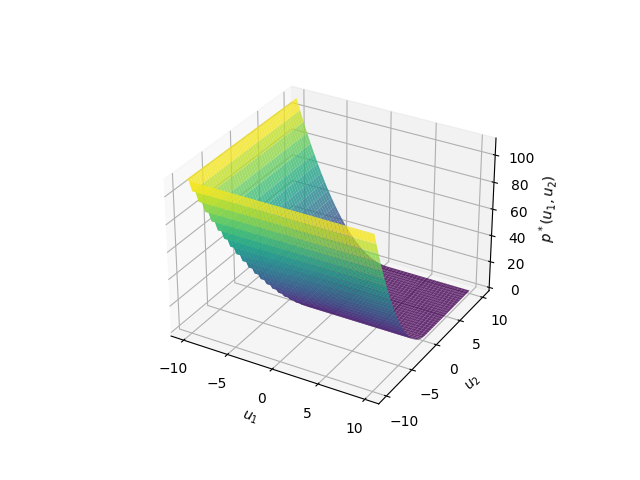
\includegraphics[scale=1]{./figs/p.png}
\end{figure}
\subsection*{(e)}
From above graph it seems like $p^*(u_1, u_2)$ is a convex function.
\subsection*{(f)}
Numerically derivated at the given point is 0.
\begin{figure}[H]
	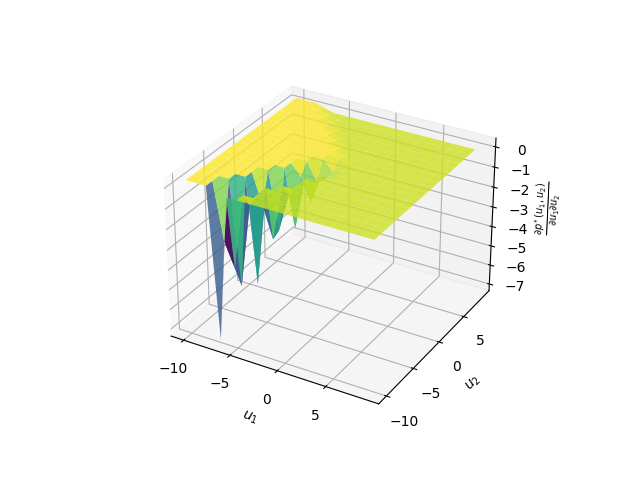
\includegraphics[scale=1]{./figs/p_dash.png}
\end{figure}
\end{document}